\documentclass{standalone}
\usepackage{tikz}
\usetikzlibrary{patterns, positioning}

\begin{document}
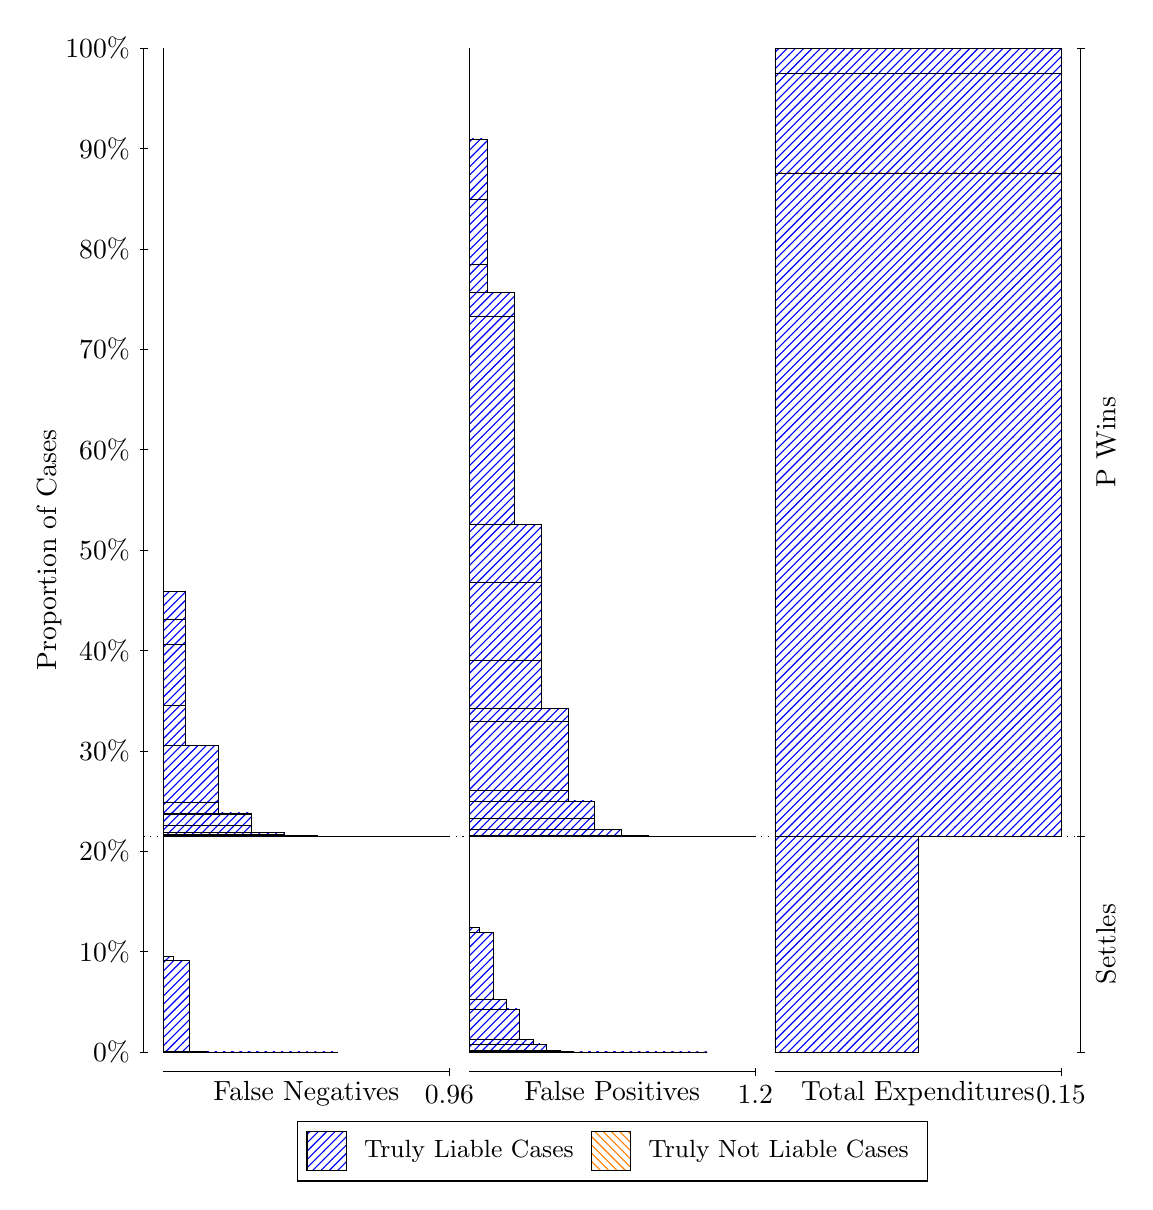
\begin{tikzpicture}
\draw[black, very thin] (1.5,1.75) -- (1.5,14.5);
\node[rotate=90, anchor=center] at (0.3, 8.125) {Proportion of Cases};
\draw[black, very thin] (1.45,1.75) -- (1.55,1.75);
\node[anchor=east] at (1.45, 1.75) {0\%};
\draw[black, very thin] (1.45,3.025) -- (1.55,3.025);
\node[anchor=east] at (1.45, 3.025) {10\%};
\draw[black, very thin] (1.45,4.3) -- (1.55,4.3);
\node[anchor=east] at (1.45, 4.3) {20\%};
\draw[black, very thin] (1.45,5.575) -- (1.55,5.575);
\node[anchor=east] at (1.45, 5.575) {30\%};
\draw[black, very thin] (1.45,6.85) -- (1.55,6.85);
\node[anchor=east] at (1.45, 6.85) {40\%};
\draw[black, very thin] (1.45,8.125) -- (1.55,8.125);
\node[anchor=east] at (1.45, 8.125) {50\%};
\draw[black, very thin] (1.45,9.4) -- (1.55,9.4);
\node[anchor=east] at (1.45, 9.4) {60\%};
\draw[black, very thin] (1.45,10.675) -- (1.55,10.675);
\node[anchor=east] at (1.45, 10.675) {70\%};
\draw[black, very thin] (1.45,11.95) -- (1.55,11.95);
\node[anchor=east] at (1.45, 11.95) {80\%};
\draw[black, very thin] (1.45,13.225) -- (1.55,13.225);
\node[anchor=east] at (1.45, 13.225) {90\%};
\draw[black, very thin] (1.45,14.5) -- (1.55,14.5);
\node[anchor=east] at (1.45, 14.5) {100\%};

\draw[black, very thin] (13.4,1.75) -- (13.4,14.5);
\draw[black, very thin] (13.35,1.75) -- (13.45,1.75);
\node[anchor=west] at (13.35, 1.75) {};
\draw[black, very thin] (13.35,4.4915) -- (13.45,4.4915);
\node[anchor=west] at (13.35, 4.4915) {};
\draw[black, very thin] (13.35,14.5) -- (13.45,14.5);
\node[anchor=west] at (13.35, 14.5) {};

\draw[black, very thin, pattern color=blue, pattern=north east lines] (1.75,1.75) rectangle (3.9677,1.75);
\draw[black, very thin, pattern color=blue, pattern=north east lines] (1.75,1.75) rectangle (3.5483,1.75);
\draw[black, very thin, pattern color=blue, pattern=north east lines] (1.75,1.75) rectangle (3.1289,1.75);
\draw[black, very thin, pattern color=blue, pattern=north east lines] (1.75,1.75) rectangle (3.024,1.75);
\draw[black, very thin, pattern color=blue, pattern=north east lines] (1.75,1.75) rectangle (2.7095,1.7503);
\draw[black, very thin, pattern color=blue, pattern=north east lines] (1.75,1.7503) rectangle (2.6046,1.7503);
\draw[black, very thin, pattern color=blue, pattern=north east lines] (1.75,1.7503) rectangle (2.29,1.7576);
\draw[black, very thin, pattern color=blue, pattern=north east lines] (1.75,1.7576) rectangle (2.1852,1.7576);
\draw[black, very thin, pattern color=blue, pattern=north east lines] (1.75,1.7576) rectangle (2.0803,2.9095);
\draw[black, very thin, pattern color=blue, pattern=north east lines] (1.75,2.9095) rectangle (1.8706,2.9683);
\draw[black, very thin, pattern color=blue, pattern=north east lines] (1.75,2.9683) rectangle (1.7657,2.9684);
\draw[black, very thin, pattern color=orange, pattern=north west lines] (1.75,2.9684) rectangle (1.75,2.9684);
\draw[black, very thin, pattern color=blue, pattern=north east lines] (1.75,2.9684) rectangle (1.75,4.4915);
\draw[black, very thin, pattern color=blue, pattern=north east lines] (1.75,4.4915) rectangle (5.3833,4.4915);
\draw[black, very thin, pattern color=blue, pattern=north east lines] (1.75,4.4915) rectangle (4.9639,4.4915);
\draw[black, very thin, pattern color=blue, pattern=north east lines] (1.75,4.4915) rectangle (4.9639,4.4915);
\draw[black, very thin, pattern color=blue, pattern=north east lines] (1.75,4.4915) rectangle (4.5445,4.4915);
\draw[black, very thin, pattern color=blue, pattern=north east lines] (1.75,4.4915) rectangle (4.125,4.4919);
\draw[black, very thin, pattern color=blue, pattern=north east lines] (1.75,4.4919) rectangle (3.7056,4.4948);
\draw[black, very thin, pattern color=blue, pattern=north east lines] (1.75,4.4948) rectangle (3.7056,4.4969);
\draw[black, very thin, pattern color=blue, pattern=north east lines] (1.75,4.4969) rectangle (3.2862,4.5155);
\draw[black, very thin, pattern color=blue, pattern=north east lines] (1.75,4.5155) rectangle (3.2862,4.5418);
\draw[black, very thin, pattern color=blue, pattern=north east lines] (1.75,4.5418) rectangle (2.8667,4.6325);
\draw[black, very thin, pattern color=blue, pattern=north east lines] (1.75,4.6325) rectangle (2.8667,4.7687);
\draw[black, very thin, pattern color=blue, pattern=north east lines] (1.75,4.7687) rectangle (2.8667,4.7877);
\draw[black, very thin, pattern color=blue, pattern=north east lines] (1.75,4.7877) rectangle (2.4473,4.9275);
\draw[black, very thin, pattern color=blue, pattern=north east lines] (1.75,4.9275) rectangle (2.4473,5.647);
\draw[black, very thin, pattern color=blue, pattern=north east lines] (1.75,5.647) rectangle (2.0279,6.1505);
\draw[black, very thin, pattern color=blue, pattern=north east lines] (1.75,6.1505) rectangle (2.0279,6.9219);
\draw[black, very thin, pattern color=blue, pattern=north east lines] (1.75,6.9219) rectangle (2.0279,7.2393);
\draw[black, very thin, pattern color=blue, pattern=north east lines] (1.75,7.2393) rectangle (2.0279,7.5982);
\draw[black, very thin, pattern color=orange, pattern=north west lines] (1.75,7.5982) rectangle (1.75,7.5982);
\draw[black, very thin, pattern color=blue, pattern=north east lines] (1.75,7.5982) rectangle (1.75,14.5);
\draw[black, very thin, pattern color=orange, pattern=north west lines] (5.6333,1.75) rectangle (8.6547,1.75);
\draw[black, very thin, pattern color=blue, pattern=north east lines] (5.6333,1.75) rectangle (8.6547,1.75);
\draw[black, very thin, pattern color=blue, pattern=north east lines] (5.6333,1.75) rectangle (8.3148,1.75);
\draw[black, very thin, pattern color=blue, pattern=north east lines] (5.6333,1.75) rectangle (7.9748,1.75);
\draw[black, very thin, pattern color=orange, pattern=north west lines] (5.6333,1.75) rectangle (7.8898,1.75);
\draw[black, very thin, pattern color=blue, pattern=north east lines] (5.6333,1.75) rectangle (7.8898,1.75);
\draw[black, very thin, pattern color=blue, pattern=north east lines] (5.6333,1.75) rectangle (7.6349,1.75);
\draw[black, very thin, pattern color=blue, pattern=north east lines] (5.6333,1.75) rectangle (7.5499,1.75);
\draw[black, very thin, pattern color=blue, pattern=north east lines] (5.6333,1.75) rectangle (7.2949,1.7503);
\draw[black, very thin, pattern color=blue, pattern=north east lines] (5.6333,1.7503) rectangle (7.2099,1.7503);
\draw[black, very thin, pattern color=orange, pattern=north west lines] (5.6333,1.7503) rectangle (7.1249,1.7503);
\draw[black, very thin, pattern color=blue, pattern=north east lines] (5.6333,1.7503) rectangle (7.1249,1.7507);
\draw[black, very thin, pattern color=blue, pattern=north east lines] (5.6333,1.7507) rectangle (6.9549,1.7586);
\draw[black, very thin, pattern color=blue, pattern=north east lines] (5.6333,1.7586) rectangle (6.8699,1.7586);
\draw[black, very thin, pattern color=blue, pattern=north east lines] (5.6333,1.7586) rectangle (6.785,1.7664);
\draw[black, very thin, pattern color=blue, pattern=north east lines] (5.6333,1.7664) rectangle (6.615,1.8513);
\draw[black, very thin, pattern color=blue, pattern=north east lines] (5.6333,1.8513) rectangle (6.53,1.8514);
\draw[black, very thin, pattern color=blue, pattern=north east lines] (5.6333,1.8514) rectangle (6.445,1.9104);
\draw[black, very thin, pattern color=blue, pattern=north east lines] (5.6333,1.9104) rectangle (6.275,2.2983);
\draw[black, very thin, pattern color=blue, pattern=north east lines] (5.6333,2.2983) rectangle (6.19,2.2984);
\draw[black, very thin, pattern color=blue, pattern=north east lines] (5.6333,2.2984) rectangle (6.105,2.4197);
\draw[black, very thin, pattern color=blue, pattern=north east lines] (5.6333,2.4197) rectangle (5.935,3.2732);
\draw[black, very thin, pattern color=blue, pattern=north east lines] (5.6333,3.2732) rectangle (5.8501,3.2732);
\draw[black, very thin, pattern color=blue, pattern=north east lines] (5.6333,3.2732) rectangle (5.7651,3.3321);
\draw[black, very thin, pattern color=blue, pattern=north east lines] (5.6333,3.3321) rectangle (5.6333,4.4915);
\draw[black, very thin, pattern color=orange, pattern=north west lines] (5.6333,4.4915) rectangle (9.2667,4.4915);
\draw[black, very thin, pattern color=blue, pattern=north east lines] (5.6333,4.4915) rectangle (9.2667,4.4915);
\draw[black, very thin, pattern color=orange, pattern=north west lines] (5.6333,4.4915) rectangle (8.9267,4.4915);
\draw[black, very thin, pattern color=blue, pattern=north east lines] (5.6333,4.4915) rectangle (8.9267,4.4915);
\draw[black, very thin, pattern color=orange, pattern=north west lines] (5.6333,4.4915) rectangle (8.5867,4.4915);
\draw[black, very thin, pattern color=blue, pattern=north east lines] (5.6333,4.4915) rectangle (8.5867,4.4916);
\draw[black, very thin, pattern color=blue, pattern=north east lines] (5.6333,4.4916) rectangle (8.5867,4.4916);
\draw[black, very thin, pattern color=blue, pattern=north east lines] (5.6333,4.4916) rectangle (8.2468,4.4919);
\draw[black, very thin, pattern color=orange, pattern=north west lines] (5.6333,4.4919) rectangle (8.2468,4.4919);
\draw[black, very thin, pattern color=blue, pattern=north east lines] (5.6333,4.4919) rectangle (8.2468,4.4923);
\draw[black, very thin, pattern color=orange, pattern=north west lines] (5.6333,4.4923) rectangle (7.9068,4.4923);
\draw[black, very thin, pattern color=blue, pattern=north east lines] (5.6333,4.4923) rectangle (7.9068,4.5011);
\draw[black, very thin, pattern color=orange, pattern=north west lines] (5.6333,4.5011) rectangle (7.5669,4.5011);
\draw[black, very thin, pattern color=blue, pattern=north east lines] (5.6333,4.5011) rectangle (7.5669,4.5726);
\draw[black, very thin, pattern color=blue, pattern=north east lines] (5.6333,4.5726) rectangle (7.2269,4.713);
\draw[black, very thin, pattern color=orange, pattern=north west lines] (5.6333,4.713) rectangle (7.2269,4.713);
\draw[black, very thin, pattern color=blue, pattern=north east lines] (5.6333,4.713) rectangle (7.2269,4.9391);
\draw[black, very thin, pattern color=blue, pattern=north east lines] (5.6333,4.9391) rectangle (6.8869,5.0682);
\draw[black, very thin, pattern color=orange, pattern=north west lines] (5.6333,5.0682) rectangle (6.8869,5.0682);
\draw[black, very thin, pattern color=blue, pattern=north east lines] (5.6333,5.0682) rectangle (6.8869,5.9453);
\draw[black, very thin, pattern color=blue, pattern=north east lines] (5.6333,5.9453) rectangle (6.8869,6.1122);
\draw[black, very thin, pattern color=blue, pattern=north east lines] (5.6333,6.1122) rectangle (6.547,6.7278);
\draw[black, very thin, pattern color=orange, pattern=north west lines] (5.6333,6.7278) rectangle (6.547,6.7278);
\draw[black, very thin, pattern color=blue, pattern=north east lines] (5.6333,6.7278) rectangle (6.547,7.7169);
\draw[black, very thin, pattern color=blue, pattern=north east lines] (5.6333,7.7169) rectangle (6.547,8.4484);
\draw[black, very thin, pattern color=orange, pattern=north west lines] (5.6333,8.4484) rectangle (6.207,8.4484);
\draw[black, very thin, pattern color=blue, pattern=north east lines] (5.6333,8.4484) rectangle (6.207,11.089);
\draw[black, very thin, pattern color=blue, pattern=north east lines] (5.6333,11.089) rectangle (6.207,11.393);
\draw[black, very thin, pattern color=blue, pattern=north east lines] (5.6333,11.393) rectangle (5.8671,11.752);
\draw[black, very thin, pattern color=blue, pattern=north east lines] (5.6333,11.752) rectangle (5.8671,12.584);
\draw[black, very thin, pattern color=blue, pattern=north east lines] (5.6333,12.584) rectangle (5.8671,13.345);
\draw[black, very thin, pattern color=blue, pattern=north east lines] (5.6333,13.345) rectangle (5.6333,14.5);
\draw[black, very thin, pattern color=orange, pattern=north west lines] (9.5167,1.75) rectangle (11.333,1.75);
\draw[black, very thin, pattern color=blue, pattern=north east lines] (9.5167,1.75) rectangle (11.333,4.4915);
\draw[black, very thin, pattern color=orange, pattern=north west lines] (9.5167,4.4915) rectangle (13.15,4.4915);
\draw[black, very thin, pattern color=blue, pattern=north east lines] (9.5167,4.4915) rectangle (13.15,12.914);
\draw[black, very thin, pattern color=orange, pattern=north west lines] (9.5167,12.914) rectangle (13.15,12.914);
\draw[black, very thin, pattern color=blue, pattern=north east lines] (9.5167,12.914) rectangle (13.15,14.182);
\draw[black, very thin, pattern color=orange, pattern=north west lines] (9.5167,14.182) rectangle (13.15,14.182);
\draw[black, very thin, pattern color=blue, pattern=north east lines] (9.5167,14.182) rectangle (13.15,14.5);
\draw[black, dotted] (1.5,4.4915) -- (13.4,4.4915);
\draw[black, very thin] (1.75,1.5) -- (5.3833,1.5);
\node[anchor=north] at (3.5667, 1.5) {False Negatives};
\draw[black, very thin] (5.3833,1.45) -- (5.3833,1.55);
\node[anchor=north] at (5.3833, 1.45) {0.96};

\draw[black, very thin] (5.6333,1.5) -- (9.2667,1.5);
\node[anchor=north] at (7.45, 1.5) {False Positives};
\draw[black, very thin] (9.2667,1.45) -- (9.2667,1.55);
\node[anchor=north] at (9.2667, 1.45) {1.2};

\draw[black, very thin] (9.5167,1.5) -- (13.15,1.5);
\node[anchor=north] at (11.333, 1.5) {Total Expenditures};
\draw[black, very thin] (13.15,1.45) -- (13.15,1.55);
\node[anchor=north] at (13.15, 1.45) {0.15};

\node[black, centered, rotate=90] at (13.72, 3.1208) {Settles};
\node[black, centered, rotate=90] at (13.72, 9.4958) {P Wins};

\draw (7.449999999999999,1.5) node[draw=none] (baseCoordinate) {};
\begin{scope}[align=center]
        \matrix[scale=0.5, draw=black, below=0.5cm of baseCoordinate, nodes={draw}, column sep=0.1cm]{
            \node[rectangle, draw, minimum width=0.5cm, minimum height=0.5cm, pattern=north east lines, pattern color=blue] {}; &
            \node[draw=none, font=\small] (B) {Truly Liable Cases}; &
            \node[rectangle, draw, minimum width=0.5cm, minimum height=0.5cm, pattern=north west lines, pattern color=orange] {}; &
            \node[draw=none, font=\small] (B) {Truly Not Liable Cases}; \\
            };
\end{scope}

\end{tikzpicture}
\end{document}